\documentclass[PhD-Yoann-Dupont.tex]{subfiles}
\begin{document}

Multir \citep{hoffmann2011knowledge} est un outil permettant d'effectuer la reconnaissance de relations entre entités à l'aide de la supervision distante \citep{mintz2009distant}, cette section se base sur l'article orginal de Multir. \citet{hoffmann2011knowledge} émet l'hypothèse que différentes phrases peuvent exprimer différentes relations pour le même couple d'entités, comme par exemple «\ Steve Jobs\ » et «\ Apple inc.\ » pour lesquelles on peut exprimer au choix la relation de fondateur ou de directeur. Sa proposition combine les deux éléments suivants :

\begin{itemize}
\item l'extraction de relation(s) au niveau du corpus, c'est-à-dire les relations entre deux entités données. Si l'on se réfère à l'exemple précédent, les relations à donner serait \emph{fondateur} et \emph{directeur}.
\item l'extraction d'une relation entre deux mentions d'entités (voir la figure \ref{fig:relation-extraction-example}), c'est-à-dire la relation exprimée entre deux mentions dans un pan de texte donné, ou la valeur \emph{nulle} si aucune relation n'est exprimée à cet endroit particulier.
\end{itemize}

Multir prend en entrée :
\begin{enumerate}
    \item $\mathcal{C}$, un corpus d'entrainement;
    \item $E$, un ensemble d'entités mentionnées dans $\mathcal{C}$, par exemple «\ Steve Jobs\ » ou «\ Apple\ »;
    \item $R$, un ensemble de relations portant un nom, par exemple "fondateur", "date de naissance";
    \item $\Delta$, un ensemble de \emph{faits}, ici de la forme $r(e) = r(e_{1},e_{2})$ tels que $r \in R$ et $e_{1},e_{2} \in E$\footnote{techniquement, Multir n'est pas limité aux relations binaires, mais nous nous y limiterons ici.};
\end{enumerate}
et donne en sortie un modèle pour effectuer l'extraction.

Multir est un modèle graphique non dirigé modélisant la probabilité jointe, entre les décisions à l'échelle du corpus et celles à l'échelle de la phrase, illustré dans le dessin de gauche dans la figure \ref{fig:YZDependencies}. Pour chaque paire d'entités $e = (e_{1},e_{2}) \in E \times E$ il existe des connexions dans le modèle pour représenter chaque instance d'une relation sur $e$. Il y a une variable booléenne de sortie $Y^{r} \forall r \in R$, représentant si un fait $r(e)$ est vérifié. Si aucune relation ne lie la paire d'entités $e$, $Y^{r}$ vaudra alors 0 pour l'ensemble des $r \in R$. Cet ensemble de classifieurs binaires permet de modéliser de multiples relations pour un même couple d'entités $e$.

Soit $\mathcal{C}_{(e_{1},e_{2})}$ l'ensembles des phrases de $\mathcal{C}$ où $e_{1}$ et $e_{2}$ sont mentionnées. Pour chaque $x_{i} \in \mathcal{C}_{(e_{1},e_{2})}$ il existe une variable latente $Z_{i}$ pour chaque $r \in R$ et la valeur \emph{nulle} (si l'instance n'exprime pas de relation connue). Un exemple de réseau instancié est donné à droite dans la figure \ref{fig:YZDependencies}.

\begin{figure}[ht!]
    \begin{minipage}{0.25\linewidth}
        \centering
        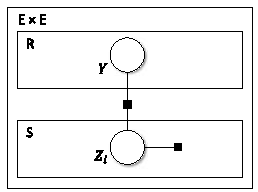
\includegraphics[scale=1.0]{images/multir/model}
    \end{minipage}
    \begin{minipage}{0.74\linewidth}
        \centering
        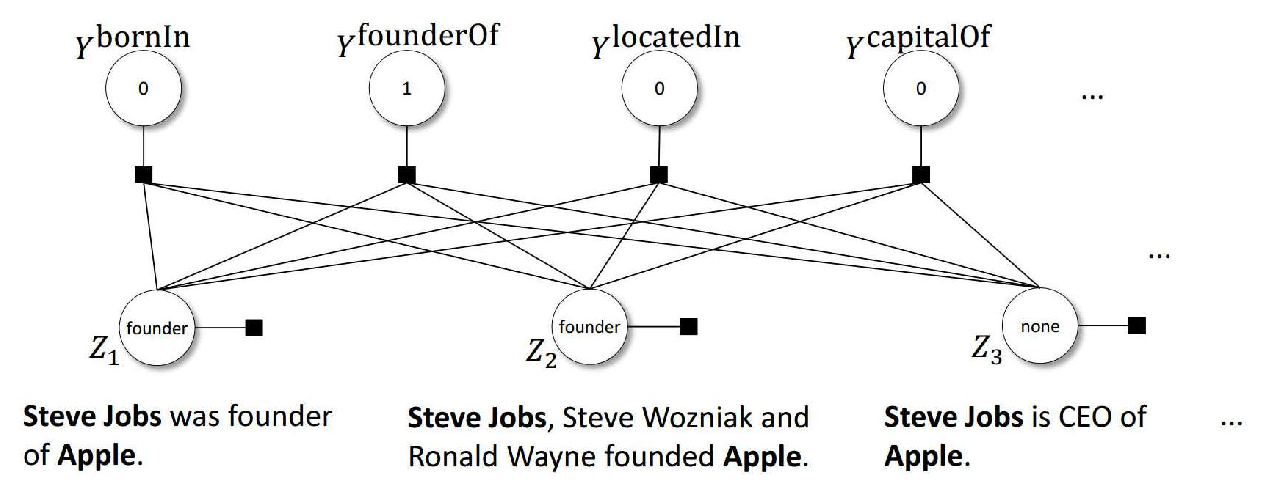
\includegraphics[scale=0.50]{images/multir/variableDependencies}
    \end{minipage}
\caption{À gauche, le modèle Multir représenté de manière générique. À droite, un exemple d'instanciation du réseau pour la paire d'entités «\ Steve Jobs\ » et «\ Apple\ ». Chaque $Z_{i}$ représente la relation à l'échelle de la phrase, tandis que les $Y^{j}$ représentent les relations à l'échelle du corpus. Exemple tiré de \citet{hoffmann2011knowledge}.}
\label{fig:YZDependencies}
\end{figure}

Concrètement, le modèle combine une probabilité conditionelle jointe sur deux variables aléatoires :
\begin{itemize}
\item \emph{Y}, la variable modélisant l'ensemble des relations entre deux entités à l'échelle du corpus;
\item \emph{Z}, la variable modélisant l'ensemble des relations entre deux mentions d'entités à l'échelle de la phrase
\end{itemize}
définie par l'équation\ \ref{eq:joint-conditional-probability}.

\begin{equation} \label{eq:joint-conditional-probability}
\begin{aligned}
p(Y=y,Z=z|x;\theta) = \frac{1}{Z_x} & \prod_r \phi^{join} (y^r,z) \\
                                    & \prod_i\phi^{extract} (z_i,x_i)
\end{aligned}
\end{equation}

Où Z$_{x}$ est un facteur de normalisation, $\phi^{join}$ une fonction caractéristique telle que définie dans l'équation\ \ref{eq:phi-join} qui s'assure qu'au moins une phrase représente un fait $r(e)$ :

\begin{equation} \label{eq:phi-join}
\phi^{join} (y^r,z) = \left\{
  \begin{array}{lr}
    1\ si\ y^r=vrai\ \wedge \exists\ i\ :\ z_i\ =\ r\ \\
    0\ sinon
  \end{array}
\right.
\end{equation}

et $\phi^{extract}$, qui prend la forme :

\begin{equation} \label{eq:phi-extract}
\phi^{extract} (z_{i},x_{i}) = \exp \left( \sum_{j} \theta_{j} \phi_{j} (z_{i},x_{i}) \right)
\end{equation}

Où chaque $\phi_{j}$ est une fonction feature similaire aux $f_{k}$ des CRF dans l'équation \ref{eq:general-CRF}. Elle vaut 1 si une configuration entre l'entrée $x_{i}$ et la sortie à l'échelle de la phrase $z_{i}$ est observée. Des exemples de ces fonctions caractéristiques sont données dans le tableau \ref{tab:multir-feature-function-example}.

\begin{table}[ht!]
\begin{tabular}{ll}
$\phi_{1}$ := & \textbf{si} (sortie = \{founder\} et tokens\_entre="was founder of") \textbf{renvoyer} 1 \\
              & \textbf{sinon renvoyer} 0 \\
$\phi_{2}$ := & \textbf{si} (sortie = \{founder\} et \{tokens\_entre="was founder of"+type\_e1=Person \\
              & \ \ \ \ +type\_e2=Company\}) \textbf{renvoyer} 1 \\
              & \textbf{sinon renvoyer} 0 \\
\end{tabular}
\caption{Exemples de fonction feature pour le premier exemple de la figure \ref{fig:YZDependencies}.}
\label{tab:multir-feature-function-example}
\end{table}

%\subsubsection{L'entrainement}
À l'entrainement, Multir prend les entrées définies plus haut. Le corpus étant construit de manière semi-automatique selon une base de faits $\Delta$, il traite les variables pour l'extraction au niveau de la phrase $Z_{i}$ comme étant latentes, les variables $Y^{r}$ de $Y$ ne sont pas observées directement, mais déduites de $\Delta$. L'ensemble d'apprentissage est défini comme étant un ensemble de paires $\{(x_{i},y_{i}) | i = 1,..,n\}$ où $i$ est l'indice d'une paire d'entités $(e_{j},e_{k})$, $x_{i}$ est alors $\mathcal{C}_{(e_{j},e_{k})}$, $y_{i}$ est un vecteur de booléens où le j-ième élément vaut 1 si $r_{j}(e_{j},e_{k}) \in \Delta$, 0 sinon. Le but est de trouver la configuration des paramètres $\theta$ maximisant la vraisemblance :

\begin{equation} \label{eq:multir-likelihood}
L(\theta) = \prod_{i} p(y_{i}|x_{i};\theta) = \prod_{i} \sum_{x} p(y_{i},z|x_{i};\theta)
\end{equation}

Cet objectif étant complexe et passant mal à l'échelle, deux approximations. La première est que l'entrainement se fait en ligne en itérant sur chaque tuple $(x_{i},y_{i})$, plutôt que d'estimer l'objectif global. La seconde est d'utiliser une approximation de Viterbi où, à chaque instant, seule la sortie la plus probable est calculée, le modèle ne sera alors mis à jour que par rapport à cette prédiction. L'algorithme \ref{alg:multir-algorithm} détaille la procédure.

\begin{algorithm}[ht!]
\caption{Algorithme d'entrainement de Multir}
\label{alg:multir-algorithm}
\begin{algorithmic}
    \Function{Entrainement}{$\mathcal{C},E,R,\Delta$}
    \State \Comment{\parbox[t]{.90\linewidth}{soit l'ensemble d'apprentissage $\{(x_{i},y_{i}) | i = 1,..,n\}$ où $i$ est l'indice d'une paire d'entités $(e_{j},e_{k})$, $x_{i}$ est alors $\mathcal{C}_{(e_{j},e_{k})}$, $y_{i}$ est un vecteur de booléens en sortie.}}
    \State initialiser vecteur $\theta$ $\gets$ 0;
    \For{$t \in 1..T$}\Comment{nombre d'itérations}
        \For{$i \in 1..n$}
            \State $(y',z') \gets \argmax{y,z}\ p(y,z | x_{i} ; \theta)$;
            \If{$y'$ $\neq$ $y_{i}$}
                \State $z^{*} \gets \argmax{z}\ p(z|x_{i},y_{i};\theta)$;
                \State $\theta \gets \theta + \phi(x_{i},z^{*}) - \phi(x_{i},z')$;
            \EndIf;
        \EndFor;
    \EndFor;
    \State \Return $\theta$;
    \EndFunction;
\end{algorithmic}
\end{algorithm}

%\subsubsection{Inférence}
Dans le cadre de KBP, nous n'avons pas utilisé l'inférence à l'échelle du corpus, c'est-à-dire $Y$, nous nous sommes contentés d'inférer les relations à l'échelle de la phrase, autrement dit $Z$. Des algorithmes étaient utilisés plus tard pour regrouper les mentions sous la même entité (multir ne regroupe les mention qu'à l'aide de leur forme de surface) dans SFV.

\end{document}